\subsection{Ergebnisse}

\subsubsection*{Teilnehmer}



\subsubsection*{Einfluss der Erklärungen auf die }

\begin{figure}[bth]
    \text{Evaluation der Positionsbestimmung}\\
    \subfloat[Berechnete und reale Koordinaten pro Achse]
    {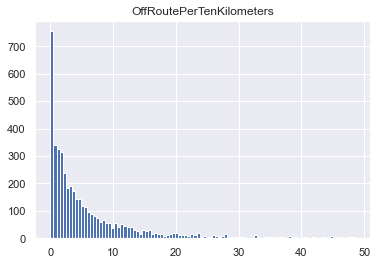
\includegraphics[width=.47\linewidth]{contents/06_model_evaluation/res/Offroute_Distribution_NE.png}}
    \hspace{5mm}
    \subfloat[Berechneter und realer Abstand]
    {
     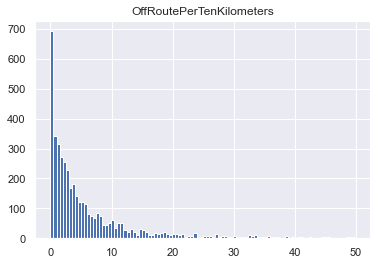
\includegraphics[width=.47\linewidth]{contents/06_model_evaluation/res/Offroute_Distribution_BN.png}} \\
    \subfloat[Berechnete und reale Koordinaten]
    {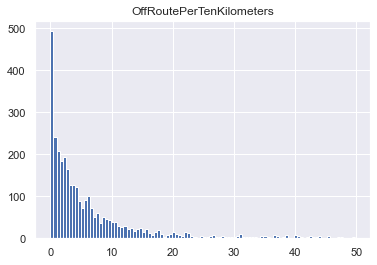
\includegraphics[width=.47\linewidth]{contents/06_model_evaluation/res/Offroute_Distribution_DN.png}}
    \hspace{5mm}
    \subfloat[Relativer Rechenfehler]
    {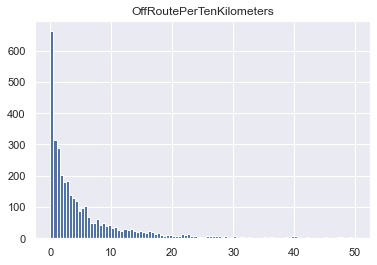
\includegraphics[width=.47\linewidth]{contents/06_model_evaluation/res/Offroute_Distribution_BDN.png}}
    \caption[Evaluation der Positionsbestimmung mithilfe des Coulombschen Gesetzes]{Evaluation der Positionsbestimmung mithilfe des Coulombschen Gesetzes bei Verwendung eines Magneten mit Magnetisierungsgrad N48, 8 mm Durchmesser und 20 mm Länge}
    \label{fig:magnetEvaluation1}
\end{figure}